\documentclass[aspectratio=169,11pt]{beamer}

% ---------- Theme Colors (matching ELTE-style design) ----------
\definecolor{UNBBlue}{RGB}{0,40,85}
\definecolor{UNBLightBlue}{RGB}{100,150,200}
\definecolor{UNBGray}{RGB}{128,128,128}
\definecolor{UNBLightGray}{RGB}{240,240,240}

% ---------- Theme Configuration ----------
\usetheme{Madrid}
\usecolortheme{default}

% Color Customization
\setbeamercolor{palette primary}{bg=UNBBlue,fg=white}
\setbeamercolor{palette secondary}{bg=UNBLightBlue,fg=white}
\setbeamercolor{palette tertiary}{bg=UNBBlue,fg=white}
\setbeamercolor{palette quaternary}{bg=UNBBlue,fg=white}
\setbeamercolor{structure}{fg=UNBBlue}
\setbeamercolor{frametitle}{bg=UNBBlue,fg=white}
\setbeamercolor{title}{bg=UNBBlue,fg=white}
\setbeamercolor{block title}{bg=UNBBlue,fg=white}
\setbeamercolor{block body}{bg=UNBLightGray,fg=black}

% Font Settings
\setbeamerfont{title}{size=\Large,series=\bfseries}
\setbeamerfont{frametitle}{size=\large,series=\bfseries}
\setbeamerfont{block title}{size=\normalsize,series=\bfseries}

% Remove navigation symbols
\setbeamertemplate{navigation symbols}{}

% Custom footer
\setbeamertemplate{footline}{
  \leavevmode%
  \hbox{%
    \begin{beamercolorbox}[wd=.3\paperwidth,ht=2.25ex,dp=1ex,center]{author in head/foot}%
      \usebeamerfont{author in head/foot}\insertshortauthor
    \end{beamercolorbox}%
    \begin{beamercolorbox}[wd=.4\paperwidth,ht=2.25ex,dp=1ex,center]{title in head/foot}%
      \usebeamerfont{title in head/foot}\insertshorttitle
    \end{beamercolorbox}%
    \begin{beamercolorbox}[wd=.3\paperwidth,ht=2.25ex,dp=1ex,right]{date in head/foot}%
      \usebeamerfont{date in head/foot}\insertshortdate{}\hspace*{2em}
      \insertframenumber{} / \inserttotalframenumber\hspace*{2ex}
    \end{beamercolorbox}}%
  \vskip0pt%
}

% ---------- Packages ----------
\usepackage[utf8]{inputenc}
\usepackage[T1]{fontenc}
\usepackage{lmodern}
\usepackage{amsmath, amssymb}
\usepackage{booktabs}
\usepackage{graphicx}
\usepackage{ragged2e}
\usepackage{tikz}
\usepackage{array}
\usepackage{xcolor}
\usepackage{multicol}
\usetikzlibrary{positioning, shapes, arrows, fit, backgrounds}

% ---------- Metadata ----------
\title[Lead-Time-Aware Predictive Incident Detection]{Lead-Time-Aware Predictive Incident Detection\\Using KPI Metrics and Logs}
\author[Akin, Alfarizy, Hanyurwimfura]{Akinbobola Akin \and Alfarizy Alfarizy \and Ishimwe Pacis Hanyurwimfura}
\institute[UNB]{University of New Brunswick \\ CS6905 -- Cloud Information Management Systems}
\date[Mar 2026]{March 2026}

% ---------- Optional spacing ----------
\setlength{\leftmargini}{1.2em}

\begin{document}

% ===== SLIDE 1: TITLE =====
\begin{frame}
\titlepage
\end{frame}

% ===== SLIDE 2: MOTIVATION =====
\begin{frame}{Motivation}
\framesubtitle{Why Predictive Incident Detection Matters}

\begin{columns}
\begin{column}{0.55\textwidth}
\begin{block}{The Challenge}
\begin{itemize}
    \item Modern cloud systems generate massive observability data
    \item Yet incident management remains \textbf{reactive}
    \item Alerts fire only \textbf{after degradation has already started}
    \item High false-alert rates cause \textbf{alert fatigue}
\end{itemize}
\end{block}

\vspace{0.5em}
\begin{alertblock}{Key Question}
Can we generate \textbf{reliable early warnings} before incidents begin, rather than merely reacting after threshold violations?
\end{alertblock}
\end{column}

\begin{column}{0.4\textwidth}
\centering
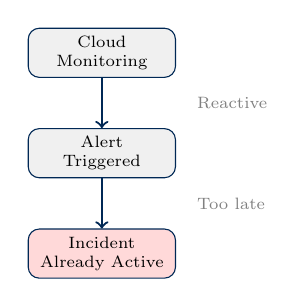
\begin{tikzpicture}[scale=0.85, transform shape,
  box/.style={rectangle, rounded corners, draw=UNBBlue, fill=UNBLightGray, minimum width=2.2cm, minimum height=0.65cm, font=\scriptsize, align=center},
  arrow/.style={->, thick, UNBBlue}
]
\node[box] (monitor) at (0,3) {Cloud\\Monitoring};
\node[box] (alert) at (0,1.5) {Alert\\Triggered};
\node[box, fill=red!15] (incident) at (0,0) {Incident\\Already Active};

\draw[arrow] (monitor) -- (alert);
\draw[arrow] (alert) -- (incident);

\node[right, font=\scriptsize, UNBGray] at (1.3,2.25) {Reactive};
\node[right, font=\scriptsize, UNBGray] at (1.3,0.75) {Too late};
\end{tikzpicture}
\end{column}
\end{columns}
\end{frame}

% ===== SLIDE 3: RESEARCH OBJECTIVE + DATASET (MERGED) =====
\begin{frame}{Research Objective \& Dataset}
\framesubtitle{Lead-Time-Aware Prediction on AIOps KPI Data}

\begin{columns}
\begin{column}{0.5\textwidth}
\begin{block}{Research Question}
How early can a model issue a reliable warning before incident onset?
\end{block}

\vspace{0.3em}
\begin{itemize}
    \item Reformulate detection as a \textbf{lead-time-aware prediction task}
    \item Horizons evaluated: \textbf{5, 10, 15 minutes}
    \item Goal: balance \textbf{precision}, \textbf{recall}, and \textbf{timeliness}
\end{itemize}

\vspace{0.3em}
{\small
\[
\text{Lead Time} = T_{\text{incident}} - T_{\text{alert}}
\]
}
\end{column}

\begin{column}{0.45\textwidth}
\begin{block}{AIOps KPI Dataset}
{\small
\begin{tabular}{ll}
\toprule
\textbf{Property} & \textbf{Value} \\
\midrule
Size & 2.4M timesteps \\
KPIs & 26 service metrics \\
Sampling & 1-min \& 5-min \\
Labels & Expert-annotated \\
\bottomrule
\end{tabular}
}
\end{block}

\vspace{0.3em}
\begin{alertblock}{Key Design Choice}
{\small Labels shifted by $H$ minutes to create \textbf{forward-looking} prediction targets}
\end{alertblock}
\end{column}
\end{columns}
\end{frame}

% ===== SLIDE 4: METHOD OVERVIEW =====
\begin{frame}{Method Overview}
\framesubtitle{Pipeline from Raw KPIs to Lead-Time Evaluation}

\centering
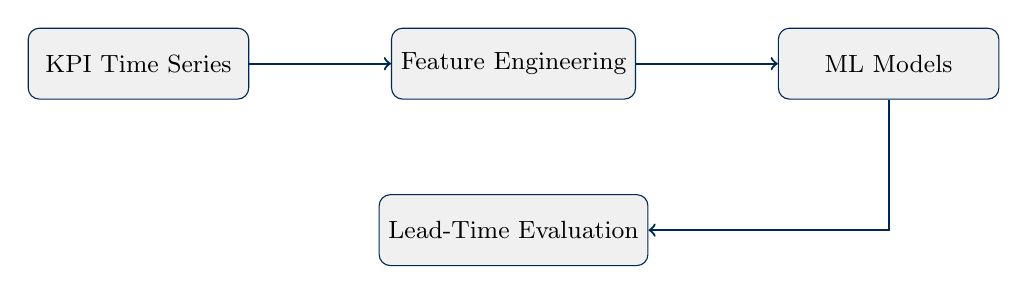
\begin{tikzpicture}[node distance=1.8cm, every node/.style={font=\small},
  box/.style={rectangle, rounded corners, draw=UNBBlue, fill=UNBLightGray, minimum width=2.8cm, minimum height=0.9cm, align=center},
  arrow/.style={->, thick, UNBBlue}
]
    \node[box] (kpi) {KPI Time Series};
    \node[box, right=of kpi] (feat) {Feature Engineering};
    \node[box, right=of feat] (model) {ML Models};
    \node[box, below=1.2cm of feat] (eval) {Lead-Time Evaluation};

    \draw[arrow] (kpi) -- (feat);
    \draw[arrow] (feat) -- (model);
    \draw[arrow] (model) |- (eval);
\end{tikzpicture}

\vspace{0.8em}
\begin{columns}[T]
\begin{column}{0.45\textwidth}
\begin{block}{KPI Statistical Features}
{\small
\begin{itemize}
    \item Rolling mean, max, std
    \item Rolling slope
    \item First difference
\end{itemize}
}
\end{block}
\end{column}
\begin{column}{0.45\textwidth}
\begin{block}{Log-Proxy Features}
{\small
\begin{itemize}
    \item Error rate
    \item Warning rate
    \item Severity-change flag
\end{itemize}
}
\end{block}
\end{column}
\end{columns}
\end{frame}

% ===== SLIDE 5: MODELS AND BASELINES =====
\begin{frame}{Models and Baselines}
\framesubtitle{Experimental Design}

\begin{columns}[T]
\begin{column}{0.48\textwidth}
\begin{block}{Predictive Models}
\begin{itemize}
    \item Gradient Boosting (GBC)
    \item Random Forest (RF)
    \item Logistic Regression (LR)
\end{itemize}
\end{block}

\vspace{0.4em}
{\small
\[
3 \text{ horizons} \times 2 \text{ feature sets} \times 3 \text{ models} = 18 \text{ configs}
\]
}

\begin{alertblock}{Calibration Target}
At most \textbf{one false alert per 24 hours per KPI}
\end{alertblock}
\end{column}

\begin{column}{0.48\textwidth}
\begin{block}{Reactive Baselines}
\begin{itemize}
    \item \textbf{Static threshold:} fixed percentile-based rule
    \item \textbf{Moving-average:} adaptive mean $\pm$ std band
\end{itemize}
\end{block}

\vspace{0.4em}
\begin{block}{Evaluation Windows}
{\small
\begin{tabular}{ll}
\toprule
\textbf{Window} & \textbf{Scope} \\
\midrule
Strict $[T{-}H, T)$ & Horizon-aware \\
Operational $[T{-}60, T)$ & Deployment \\
\bottomrule
\end{tabular}
}
\end{block}
\end{column}
\end{columns}
\end{frame}

% ===== SLIDE 6: KEY RESULTS — BAR CHARTS =====
\begin{frame}{Key Results: Method Comparison}
\framesubtitle{Operational Window $[T{-}60\text{min}, T)$}

\begin{center}

\includegraphics[width=0.92\linewidth]{comparison_bar_charts_operational.png}
\end{center}

\vspace{-0.3em}
{\small
\textbf{Takeaway:} GBC with KPI+Logs achieves the highest precision across all horizons while maintaining competitive lead time and recall.
}
\end{frame}

% ===== SLIDE 7: PRECISION VS DETECTION RATE =====
\begin{frame}{Precision vs.\ Detection Rate}
\framesubtitle{The Core Trade-off Under the Operational Window}

\begin{columns}
\begin{column}{0.55\textwidth}
\begin{center}

\includegraphics[width=\linewidth]{precision_vs_detection_operational.png}
\end{center}
\end{column}

\begin{column}{0.4\textwidth}
\begin{block}{Reading the Plot}
{\small
\begin{itemize}
    \item \textbf{Top-left} = high precision, fewer false alarms
    \item \textbf{Bottom-right} = high detection, more noise
    \item GBC KPI+Logs dominates the top-left region across all horizons
\end{itemize}
}
\end{block}

\vspace{0.3em}
\begin{alertblock}{Main Finding}
{\small Predictive models don't dramatically increase lead time, but they \textbf{substantially reduce false alerts}.}
\end{alertblock}
\end{column}
\end{columns}
\end{frame}

% ===== SLIDE 8: FEATURE IMPORTANCE =====
\begin{frame}{Feature Importance}
\framesubtitle{Gradient Boosting at $H=15$ min}

\begin{center}

\includegraphics[width=0.85\linewidth]{feature_importance_H15.png}
\end{center}

\vspace{-0.3em}
{\small
\textbf{Key insight:} The \textbf{error-rate proxy} is the second most important feature in the KPI+Logs model, confirming that log-like behavioral signals add meaningful predictive value beyond raw KPI statistics.
}
\end{frame}

% ===== SLIDE 9: EFFECT OF LOG-PROXY FEATURES =====
\begin{frame}{Effect of Log-Proxy Features}
\framesubtitle{KPI-Only vs.\ KPI+Logs at $H=15$}

\begin{columns}
\begin{column}{0.5\textwidth}
\begin{block}{Performance Improvement}
{\small Log-proxy features consistently boosted both precision and recall:}

\vspace{0.4em}
\[
\text{Recall: } 0.16 \rightarrow 0.43
\]
\[
\text{Precision: } 0.63 \rightarrow 0.91
\]
\end{block}

\vspace{0.4em}
\begin{block}{Why It Works}
{\footnotesize
\begin{itemize}
    \item Error-rate captures behavioral shifts invisible to raw KPIs
    \item Severity-change flag detects mode transitions
    \item Complements statistical features with semantic signals
\end{itemize}
}
\end{block}
\end{column}

\begin{column}{0.45\textwidth}
\begin{table}
\centering
\small
\begin{tabular}{lcc}
\toprule
\textbf{Method} & \textbf{Prec.} & \textbf{Rec.} \\
\midrule
GBC KPI+Logs & \textbf{0.91} & \textbf{0.43} \\
GBC KPI Only & 0.63 & 0.16 \\
Baseline Static & 0.63 & 0.47 \\
Baseline MA & 0.42 & 0.02 \\
\bottomrule
\end{tabular}
\caption{\small At $H=15$, Operational Window}
\end{table}

\vspace{0.3em}
\begin{alertblock}{Conclusion}
{\small Multi-signal fusion is essential for reliable prediction.}
\end{alertblock}
\end{column}
\end{columns}
\end{frame}

% ===== SLIDE 10: CASE STUDY — KPI VISUALIZATION =====
\begin{frame}{Case Study: KPI-Level Prediction}
\framesubtitle{GBC KPI+Logs on KPI 1c35dbf5 at $H=15$ min}

\begin{center}

\includegraphics[width=0.7\linewidth]{kpi_1c35dbf57f55f5e4_H15_GBC_KPI_PLUS_LOGS.png}
\end{center}

\vspace{-0.3em}
{\small
\textbf{Top:} Raw KPI values with ground-truth incident windows (pink).
\textbf{Bottom:} Prediction scores with calibrated threshold (red dashed). Scores rise sharply ahead of the major incident region, demonstrating effective early warning.
}
\end{frame}

% ===== SLIDE 11: CONCLUSION =====
\begin{frame}{Conclusion}
\framesubtitle{Summary of Contributions}

\begin{columns}
\begin{column}{0.6\textwidth}
\begin{block}{Key Findings}
\begin{enumerate}
    \item Reframed cloud incident detection as a \textbf{lead-time-aware prediction problem}
    \item Predictive models achieve comparable warning time with \textbf{significantly higher precision}
    \item KPI + log-proxy features \textbf{outperform} KPI-only across all settings
    \item The \textbf{error-rate proxy} emerged as a top predictive feature
\end{enumerate}
\end{block}
\end{column}

\begin{column}{0.35\textwidth}
\begin{alertblock}{Takeaway}
The main operational benefit is not much earlier alerts, but \textbf{more trustworthy alerts with less alert fatigue}.
\end{alertblock}

\vspace{0.3em}
\begin{block}{Practical Impact}
{\small
Fewer false alarms $\rightarrow$ higher on-call trust $\rightarrow$ faster incident response
}
\end{block}
\end{column}
\end{columns}
\end{frame}

% ===== SLIDE 12: FUTURE WORK =====
\begin{frame}{Future Work}
\framesubtitle{Next Steps for Research}

\begin{columns}
\begin{column}{0.5\textwidth}
\begin{block}{Technical Extensions}
\begin{itemize}
    \item Integrate real system logs (not proxies)
    \item Incorporate additional observability signals (traces, topology)
    \item Test deeper sequence models (LSTM, Transformer)
\end{itemize}
\end{block}
\end{column}

\begin{column}{0.45\textwidth}
\begin{block}{Deployment Directions}
\begin{itemize}
    \item Evaluate in live cloud monitoring environments
    \item Online model updating for concept drift
    \item Integration with existing AIOps platforms
\end{itemize}
\end{block}
\end{column}
\end{columns}
\end{frame}

% ===== SLIDE 13: THANK YOU =====
\begin{frame}

\begin{center}
\setbeamercolor{block title}{bg=UNBBlue,fg=white}
\setbeamercolor{block body}{bg=UNBBlue,fg=white}
\begin{block}{}
\centering
\textbf{Thank you for your attention!}
\end{block}

\vspace{0.3em}
{\normalsize Questions?}
\end{center}
\end{frame}

% ================================================================
% BACKUP SLIDES (for Q&A)
% ================================================================

% ===== BACKUP 1: LEAD TIME DISTRIBUTION =====
\begin{frame}{Backup: Lead Time Distribution}
\framesubtitle{Operational Window $[T{-}60\text{min}, T)$}

\begin{center}

\includegraphics[width=0.88\linewidth]{lead_time_boxplots_operational.png}
\end{center}

\vspace{-0.3em}
{\small
Predictive models achieve \textbf{comparable median lead times} to reactive baselines ($\sim$30--35 min), but with far fewer false positives --- the key operational advantage.
}
\end{frame}

% ===== BACKUP 2: STRICT WINDOW RESULTS =====
\begin{frame}{Backup: Strict Window Results}
\framesubtitle{Strict Evaluation $[T{-}H, T)$}

\begin{center}

\includegraphics[width=0.92\linewidth]{comparison_bar_charts_strict.png}
\end{center}

\vspace{-0.3em}
{\small
Under the strict window, trends are consistent: GBC KPI+Logs maintains precision advantage. Lead times are naturally capped by the horizon $H$.
}
\end{frame}

% ===== BACKUP 3: ALTERNATIVE KPI CASE =====
\begin{frame}{Backup: Alternative KPI Behavior}
\framesubtitle{GBC KPI+Logs on KPI a5bf5d65 at $H=15$ min}

\begin{center}

\includegraphics[width=0.7\linewidth]{kpi_a5bf5d65261d859a_H15_GBC_KPI_PLUS_LOGS.png}
\end{center}

\vspace{-0.3em}
{\small
A spikey KPI with sparse anomalies. The model produces elevated scores near the incident spike ($\sim$Jul 19) while keeping scores low during normal periods --- demonstrating generalization across diverse KPI behaviors.
}
\end{frame}

\end{document}